\section{Internet of Plants}

\subsection{Overview}

The Internet of Plants, also called IoP, is a concept that aims to interconnect the plant device previously built.
This in order to empower the device capabilities and to provide a better user experience.
This project includes:
\begin{itemize}
    \item A better sound quality by using professional sonification software
    \item The ability to create a full artistic experience by creating a distributed instrument
    \item Refining the interaction with the plant by using more complex data analyses
\end{itemize}



\subsection{Communication}

The communication system is based on WiFi technology. The ESP32 has specific wireless capabilities.
The server and the ESP32 devices are connected to the same network.
The ESP32 sends the raw data to the server using IP\footnote{Internet Protocol}. This is done
through a TCP \footnote{Transmission Control Protocol} socket open between the server and one ESP32.
The server can open as many socket as there are clients. The data sent using a string.
A "#" start character and a ";\\n" stop character are used to prevent the messages to 
be truncated and still processed on the server side. The IP protocol (whether it is on WiFi
or Ethernet) has been chosen for this application for several reasons:

\begin{itemize}
    \item Allow high bandwidth
    \item Available in most places
    \item Allow connection of multiple devices
    \item Already available on the server and on the ESP32
\end{itemize}

Other communication protocols have been benchmarked. Here is a table that summarizes
the choice: 

\begin{table}[h!]
    \begin{tabular}{lllll}
    Protocol                            & IP (WiFi/Ethernet) & Bluetooth & BLE   & Zigbee \\
    Handle multiple connections         & Yes                & No        & No    & Yes    \\
    Requires additional hardware        & No                 & No        & No    & Yes    \\
    Subject to interference             & Yes                & Few       & Few   & Yes    \\
    Energy efficiency (using a battery) & Days               & Months    & Years & Years 
    \end{tabular}
\end{table}

The result of this table confirms that WiFi is the right choice for our specific application.
\subsection{Server}

The server is a small fanless computer running Lubuntu. Lubuntu is a lighter version of Ubuntu
that includes LXQt as desktop environnement. The choice of a distribution with graphical
interface is induced by the use of \textit{Pure Data} as sonification software.

Pure Data (PD) is an open-source visual programming language designed primarily for 
creating interactive multimedia applications, particularly in the fields of audio, video, 
and graphical processing.
Pure Data is part of a family of patcher programming languages, which also includes Max/MSP.
Unlike traditional text-based programming, PD uses a graphical interface where users connect 
"objects" with virtual patch cables to create complex data flows and signal processing chains. 
Its modular design allows for real-time manipulation of sound and graphics, making it a powerful 
tool for artists, musicians, and researchers interested in exploring experimental media. 

Pure Data requires, in a development environnement, a graphical interface to test and debug.
The Pure Data patch receive the data through a TCP socket. The data is processed through several 
operations. Then, if a threshold is passed, an interaction happened and the music is triggered.
The music is outputted through the item \textit{DAC} which means Digital to Analog Converter. 
The digital input from pure data is converted to a sound that speakers can output.

\begin{figure}[h]
    \centering
    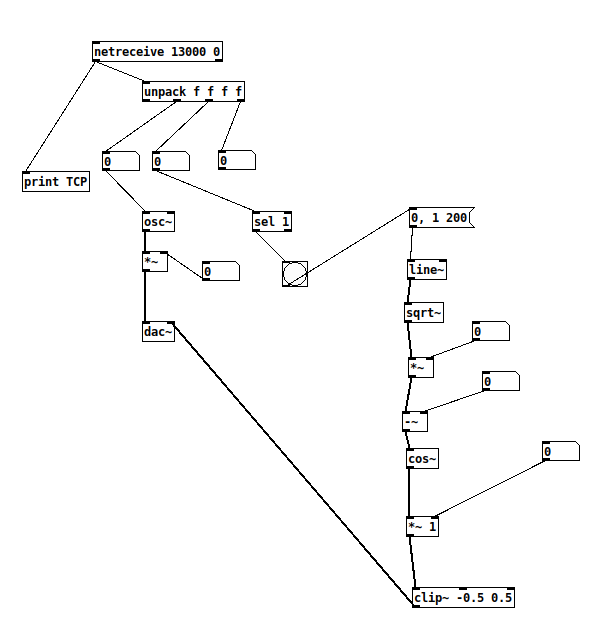
\includegraphics[width=\textwidth]{pure_data_patch.png}
    \caption{Basic \textit{Pure Data} patch that is used for sonification of the data
    of the plant. In case of an art exhibition, the Pure Data patch can be upgraded to meet the
    artist needs} 
    \vspace{0.1cm}
    \label{fig:pure_data_patch}
\end{figure}


Pure Data is a sonification software that require data as input. In order to get and process the data,
we designed a Python based software.
The software is object oriented. The standalone IoP modules connect using WiFi to the receiver module
of the software. The connection is made using TCP socket from the ESP32 to the server.
The main module of the software then creates software abstraction of the standalone module. 
The abstraction module is processing and storing all the processed data.
The main module then send the processed data to Pure Data patch using also local TCP socket.

\begin{figure}[h]
    \centering
    \includegraphics[width=\textwidth]{iop_architecture.png}
    \caption{Architecture diagram of Internet of Plants project centered on server-side.} 
    \vspace{0.1cm}
    \label{fig:server_architecture}
\end{figure}


\subsection{Deployment and application}

\subsubsection{Distributed instruments}

\subsubsection{Art exhibition}

\subsection{Conclusion}

